\documentclass[tikz,border=10pt]{standalone}
\usepackage[utf8]{inputenc}
\usepackage[T1]{fontenc}
\usepackage{amsmath,amssymb}
\usepackage{tikz}
\usetikzlibrary{shapes.geometric, arrows.meta, positioning, calc, fit, backgrounds}

\definecolor{primary}{HTML}{0F172A}
\definecolor{primaryblue}{HTML}{1E3A8A}
\definecolor{accentblue}{HTML}{0284C7}
\definecolor{tealaccent}{HTML}{0D9488}
\definecolor{darkgreen}{HTML}{065F46}
\definecolor{lightgreen}{HTML}{ECFDF5}
\definecolor{crimson}{HTML}{991B1B}
\definecolor{lightred}{HTML}{FEF2F2}
\definecolor{amber}{HTML}{B45309}
\definecolor{lightamber}{HTML}{FFFBEB}
\definecolor{boxbg}{HTML}{F8FAFC}

\begin{document}

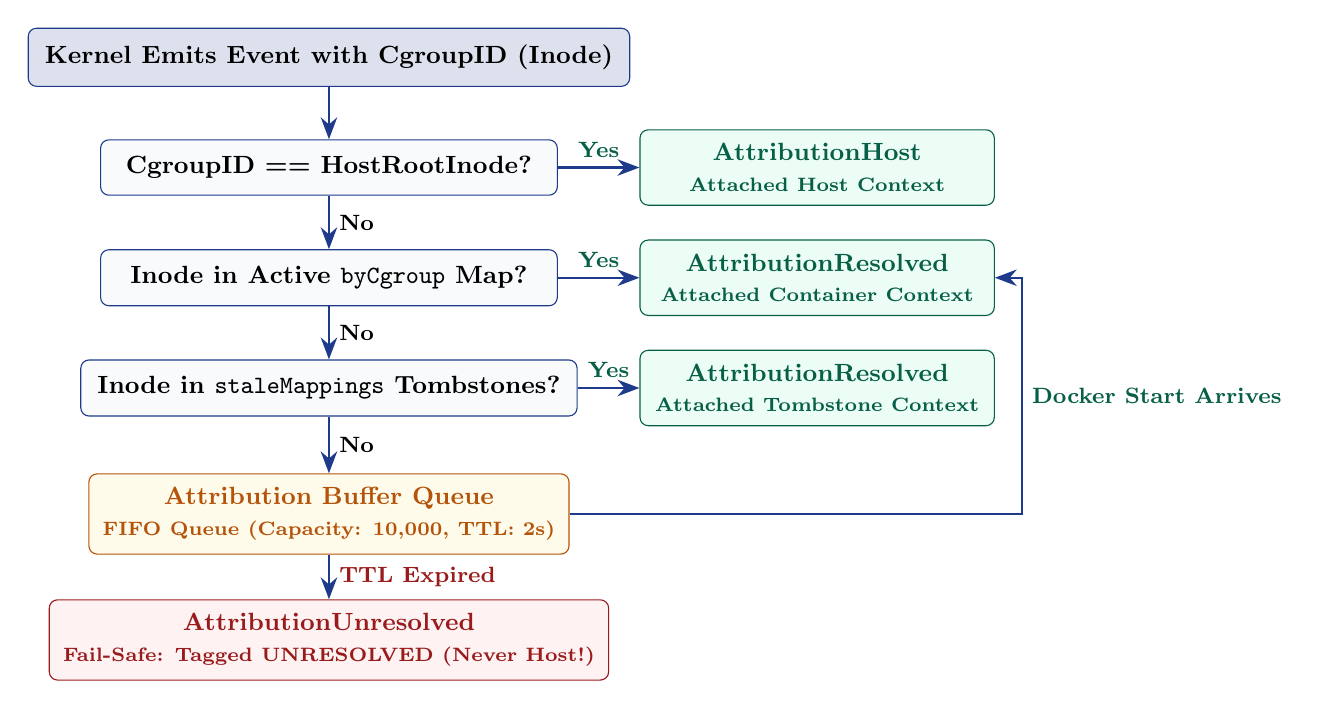
\begin{tikzpicture}[
    check/.style={rectangle, draw=primaryblue, fill=boxbg, rounded corners=3pt, font=\small\bfseries, align=center, inner sep=6pt, minimum width=5.8cm},
    resolved/.style={rectangle, draw=darkgreen, fill=lightgreen, text=darkgreen, rounded corners=3pt, font=\small\bfseries, align=center, inner sep=5pt, minimum width=4.5cm},
    pending/.style={rectangle, draw=amber, fill=lightamber, text=amber, rounded corners=3pt, font=\small\bfseries, align=center, inner sep=5pt, minimum width=5.8cm},
    failed/.style={rectangle, draw=crimson, fill=lightred, text=crimson, rounded corners=3pt, font=\small\bfseries, align=center, inner sep=5pt, minimum width=5.8cm},
    arrow/.style={-{Stealth[scale=1.2]}, thick, draw=primaryblue}
]
    \node[check, fill=primaryblue!15] (start) at (0, 5.0) {Kernel Emits Event with CgroupID (Inode)};
    \node[check] (checkhost) at (0, 3.6) {CgroupID == HostRootInode?};
    \node[resolved] (host) at (6.2, 3.6) {AttributionHost\\ \scriptsize Attached Host Context};

    \node[check] (active) at (0, 2.2) {Inode in Active \texttt{byCgroup} Map?};
    \node[resolved] (container) at (6.2, 2.2) {AttributionResolved\\ \scriptsize Attached Container Context};

    \node[check] (tomb) at (0, 0.8) {Inode in \texttt{staleMappings} Tombstones?};
    \node[resolved] (stale) at (6.2, 0.8) {AttributionResolved\\ \scriptsize Attached Tombstone Context};

    \node[pending] (queue) at (0, -0.8) {Attribution Buffer Queue\\ \scriptsize FIFO Queue (Capacity: 10,000, TTL: 2s)};
    \node[failed] (unresolved) at (0, -2.4) {AttributionUnresolved\\ \scriptsize Fail-Safe: Tagged UNRESOLVED (Never Host!)};

    \draw[arrow] (start) -- (checkhost);
    \draw[arrow] (checkhost) -- node[above, font=\footnotesize\bfseries\color{darkgreen}]{Yes} (host);
    \draw[arrow] (checkhost) -- node[right, font=\footnotesize\bfseries]{No} (active);
    \draw[arrow] (active) -- node[above, font=\footnotesize\bfseries\color{darkgreen}]{Yes} (container);
    \draw[arrow] (active) -- node[right, font=\footnotesize\bfseries]{No} (tomb);
    \draw[arrow] (tomb) -- node[above, font=\footnotesize\bfseries\color{darkgreen}]{Yes} (stale);
    \draw[arrow] (tomb) -- node[right, font=\footnotesize\bfseries]{No} (queue);
    \draw[arrow] (queue) -- node[right, font=\footnotesize\bfseries\color{crimson}]{TTL Expired} (unresolved);
    \draw[arrow] (queue.east) -- (8.8, -0.8) |- node[pos=0.25, right, font=\footnotesize\bfseries\color{darkgreen}]{Docker Start Arrives} (container.east);
\end{tikzpicture}

\end{document}
